% !TeX spellcheck = en_US
\documentclass[12pt,a4paper]{article}
\usepackage[utf8]{inputenc}
\usepackage[german]{babel}
\usepackage[T1]{fontenc}
\usepackage{amsmath}
\usepackage{amsfonts}
\usepackage{amssymb}
\usepackage{graphicx}
\usepackage[left=2.5cm,right=2.5cm,top=2cm,bottom=2cm]{geometry}
\usepackage{float}

\usepackage{subcaption}
\usepackage{siunitx}
\usepackage{verbatim} 


\author{Gruppe A2 \\ Julián Häck, Maria Spethmann}
\title{Protokoll Wellenlehre \\ Physikalisches Grundpraktikum 2}


\begin{document}
	\maketitle\thispagestyle{empty} % Keine Seitenzahl auf der Titelseite
	\newpage
	\pagestyle{headings} % Seitenzahlen oben, Section und Subsection in Kopfzeile
	\tableofcontents
	\newpage

\section{Theorie}

\textbf{Wellen} \\
Wellen sind Störungen einer Feldgröße, die in Raum und Zeit fortschreiten und ungedämpft die Wellengleichung erfüllen.
\begin{equation}
\frac{\partial^2}{\partial t^2} a(\vec{x},t)= c^2 \left(\frac{\partial^2}{\partial x^2} + \frac{\partial^2}{\partial y^2} + \frac{\partial^2}{\partial z^2}\right) a(\vec{x}, t)
\end{equation} 
Im Fall von Mikrowellen ist das elektrische Feld $\vec{E}$ bzw. das magnetische Feld $\vec{B}$ diese Feldgröße. Da die Amplitude dieser senkrecht zur Ausbreitungsrichtung der Wellen liegt, handelt es sich um transversale Wellen. Grundlage hierfür sind die Maxwellschen Gleichungen:
\begin{equation}
div\vec{D} = \rho
\end{equation}
\begin{equation}
div\vec{B} = 0
\end{equation}
\begin{equation}
rot\vec{E} = -\frac{\partial}{\partial t}\vec{B}
\end{equation}
\begin{equation}
rot\vec{H} = \frac{\partial}{\partial t}\vec{D} + \vec{j}
\end{equation}
mit
\begin{align*}
\vec{D} = \epsilon_0\vec{E} + \vec{P} \quad \text{und} \quad \vec{B} = \mu_0\vec{H} + \vec{M}
\end{align*}
mit $\epsilon_0$ und $\mu_0$ als Influenz- bzw. Induktionskonstante, Stromdichte $\vec{j}$, Ladungsdichte $\rho$, Magnetisierung $\vec{M}$ und Polarisierung $\vec{P}$. Außerdem nehmen wir näherungsweise an, dass $\vec{P},\vec{M},\rho,\vec{j}=0$.\newline
Die Phasengeschwindigkeit $c$ entspricht:
\begin{equation}
c=\frac{1}{\sqrt{\epsilon_0\epsilon_r\mu_0\mu_r}}
\end{equation}
mit der erneuten Näherung $\epsilon_r = 1 = \mu_r$.
Eine spezielle Lösung der Wellengleichung ist die harmonische ebene Welle mit 
\begin{align*}
a(x,t)=a_0 \cdot sin(\omega t \pm kx + \phi) , \quad \text{Kreisfrequenz} \, \omega = 2\pi f, \quad \text{Kreiswellenzahl} \, k= 2\pi / \lambda
\end{align*}
\textbf{Stehende Welle} \\
Stehende Wellen sind die einfachste Form der Überlagerung. Trifft eine ebene, harmonische Welle senkrecht auf einen geeigneten Reflektor, so überlagern sich die Einfallende und Reflektierte zu einer stehenden Welle. 
\begin{align*}
a(x,t)=2a_0 \cdot sin(\omega t)\cdot sin(kx)
\end{align*}
\textbf{Brechung} \\
Beim Übergang von unterschiedlich dichten Medien werden Wellen nach dem Gesetz von Snellius gebrochen.
\begin{equation}
n_1 \cdot sin(\alpha) = n_2 \cdot sin(\beta),
\end{equation}
wobei $n_1$ und $\alpha$ der Brechungsindex und der Brechungswinkel von Medium 1 sind und analog $n_2$ und $\beta$ der Brechungsindex und Brechungswinkel von Medium 2.\\\\ 
\textbf{Polarisation} \\
Transversale Wellen können polarisiert werden. Dabei gibt es die Extremfälle der zirkularen und der linearen Polarisation. Im Fall der linearen Polarisation kann die Schwingungsebene durch einen Polarisationsfilter geändert werden. Dabei sinkt die Intensität gemäß dem Gesetz von Malus:
\begin{equation}
I(\alpha) = I_0 \cdot cos^{2}(\alpha)
\end{equation}
mit dem Winkel $\alpha$ zwischen Polarisationsebene des Polarisationsfilter und der einfallenden Welle.
Im unserem Experiment sind Sender und Empfänger parallele zueinander stehende Antennendipole, wodurch sich für die Intensität
\begin{equation}
I(\alpha) = I_0 \cdot cos^{4}(\alpha)
\end{equation}
ergibt. \newline \newline
\textbf{Optischer Tunneleffekt} \\
Wird in einem kleinen Abstand $D$ hinter einem Halbzylinder, das eine einfallende Welle unter dem Winkel der Totalreflexion reflektiert, ein weiterer Halbzylinder gestellt, kann man hinter dem zweiten Halbzylinder eine transmittierte Welle messen. Dieser Effekt wird als Analogon zur Quantenmechanik Optischer Tunneleffekt genannt.
Die transmittierte Welle folgt dabei dem Intensitätsverlauf
\begin{equation}
I_T \sim exp(\frac{-2\pi D}{\lambda})
\end{equation}

\newpage

\section{Allgemeiner Versuchsaufbau}

\begin{figure}[H]
\centering
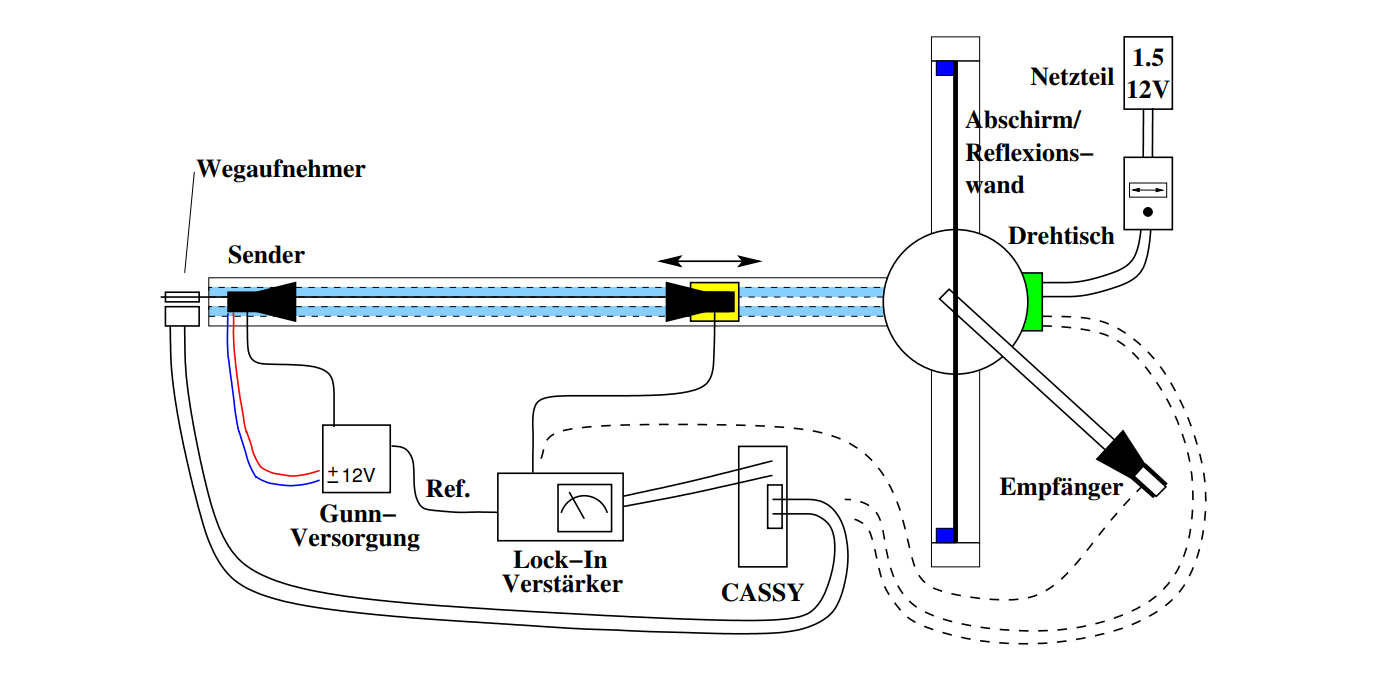
\includegraphics[scale=0.6]{Bilder/Versuchsaufbau.png}
\caption{Prinzipieller Versuchsaufbau (Quelle: Versuchshandbuch)}
\label{versuchsaufbau}
\end{figure}
Für die folgenden Versuche wird im Allgemeinen benötigt:
\begin{itemize}
\item 
Eine Gunn-Versorgung mit Modulator
\item
Ein Lock-In Messverstärker
\item
Ein Gunn Oszillator mit Hornstrahler
\item
Ein Empfänger mit Hornantenne
\item
Ein Sensor-CASSY mit Stromquellenbox LEYBOLD 542 031
\item
Ein Wegaufnehmer LEYBOLD 529 031 inklusive Faden und Gegengewicht
\item
Mehrere Kabel und Netzgeräte
\end{itemize}
Außerdem wird für bestimmte Versuche folgendes ergänzt:
\begin{itemize}
\item
Ein Polarisationsfilter
\item
Zwei PE-Halbzylinder
\item
Verschiedene Abstandsbleche
\item
Ein motorbetriebener Drehtisch
\end{itemize}
Wenn nicht anders beschrieben, erfolgt die Messwerterfassung der einzelnen Versuche unter folgenden Einstellungen (Tabelle \ref{tab:MessparameterAllgemein}).
\begin{table}[H]
	\centering
	\begin{tabular}{|c|c|}
		\hline 
		Messbereich Spannung  & -0.3 V .. 0.3 V \\ 
		\hline 
		Messbereich Widerstand Wegaufnehmer & $0\,\text{k}\Omega\ ..\ 10\,\text{k}\Omega$\\ 
		\hline 
		Messbereich Widerstand Winkelaufnehmer & $0\,\text{k}\Omega\ ..\ 10\,\text{k}\Omega$\\
		\hline
		Messwerterfassung Spannung & gemittelt über 200 ms \\ 
		\hline 
		Messwerterfassung Widerstand Wegaufnehmer & gemittelt über 200 ms \\ 
		\hline 
		Messwerterfassung Widerstand Winkelaufnehmer & gemittelt über 200 ms \\ 
		\hline
	\end{tabular} 
	\caption{Einstellungen der Messparameter}
	\label{tab:MessparameterAllgemein}
\end{table}
\newpage
\section{Kalibrierung des Wegaufnehmers}
\subsection{Versuchsbeschreibung}
Die Vermessung stehender Wellen im späteren Teilversuch erfordert die Bestimmung der genauen Entfernung zwischen Empfänger und Reflexionswand. Dazu wird ein Mehrgang-Drehpotentiometer als Wegaufnehmer verwendet, den wir in diesem Vorversuch kalibrieren.
Um nun aus dem gemessenen Widerstand die Strecke zu erhalten, benötigen wir den sich aus dem linearen Zusammenhang zwischen Widerstand und Strecke ergebenden Kalibrationsfaktor k:
\begin{align*}
S = k \cdot R + b
\end{align*}
Dieser wird in diesem Versuch bestimmt.
\subsection{Versuchsaufbau und Durchführung}
Der Schlitten des Empfängers wird mit dem Faden verbunden und dieser dann über die Rolle des Wegaufnehmers gelegt. Auf der anderen Seite des Fadens wird das Gegengewicht befestigt um den Faden gespannt zu halten. Dabei ist darauf zu achten, dass der Faden parallel zu der Führungsschiene des Schlittens läuft um Fehler durch eine Parallaxe zu vermeiden. Als Reflxionswand verwenden wir einen Polarisationsfilter, der senkrecht zur Polarisationsebene der ausgesendeten Wellen ausgerichtet ist, und somit die Welle vollständig reflektiert. \newline
Nun wird der Abstand zwischen Empfänger und Reflexionswand gegen den Widerstand des Wegaufnehmers gemessen. Dazu wird der Schlitten des Empfängers in äquidistanten Abstängen $\Delta S = 5\,\text{cm}$ verschoben. Nach jeder Verschiebung wird der Widerstand des Wegaufnehmers über 200ms gemittelt aufgezeichnet. Die Strecken werden manuell mit einem Maßband mit Millimeterskala abgelesen. 

\subsection{Versuchsauswertung}

\begin{figure}[]
\centering
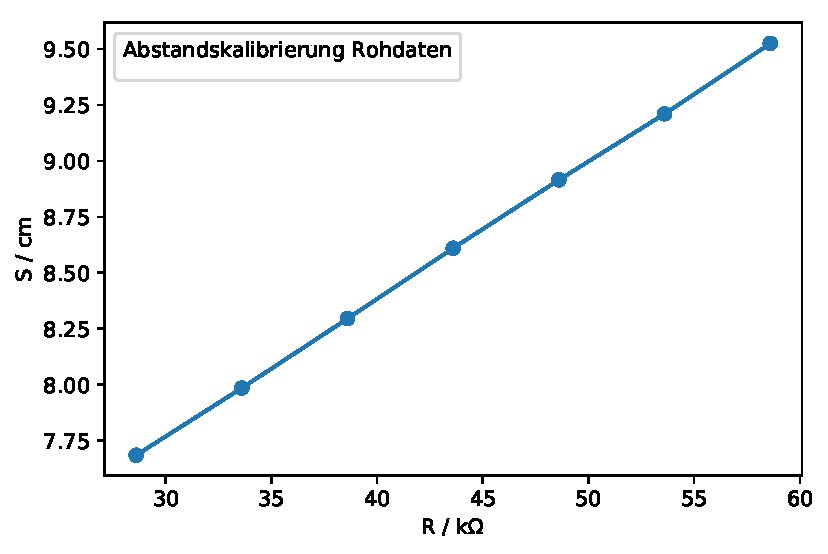
\includegraphics[scale=1]{Bilder/Abstandskal_Rohdaten.pdf}
\caption{Abstand des Empfängers zur Reflexionswand als Funktion der gemessenen Widerstände des Wegaufnehmers}
\label{Abstandskal_Rohdaten}
\end{figure}

Abb.~\ref{Abstandskal_Rohdaten} zeigt die Rohdaten unserer Messung. Mit Hilfe der linearen Regression wird nun eine Ausgleichsgerade durch die Messpunkte gelegt und deren Steigung bestimmt. Um die Korrelation zwischen der Steigung $k$ und dem y-Achsensabschnitt $b$ zu minimieren, werden die Messwerte zun"achst um ihren Mittelwert verschoben. Letztendlich erh"alt man die Strecke $S$ als Funktion des Widerstandes als
\begin{align}
S-\bar{S}=k\cdot (R-\bar{R}) + b
\end{align}
wobei $\bar{S}$ und $\bar{R}$ die Mittelwerte der gemessenen Orte bzw. Widerst"ande sind.
Dabei wurde angenommen, dass sowohl die Wegmessung mit dem Maßband als auch die Widerstandsmessung fehlerbehaftet sind mit den konstanten Unsicherheiten:
\begin{align}
\sigma_S &= \frac{1\text{mm}}{\sqrt{12}} \\
\sigma_R &= \frac{10\text{k}\Omega}{4096\cdot\sqrt{12}}
\end{align}
Der Fehler auf S ist auf die Genauigkeit des Maßbandes und der Fehler auf R auf die Digitalisierung der Widerstandsmessung mit dem Sensor Cassy zurückzuführen. Wir nehmen eine Gleichverteilung innerhalb der kleinsten Skalenbreite an.
\begin{comment}
\begin{figure}
	\centering
	\begin{subfigure}[]{\textwidth}
	\centering
	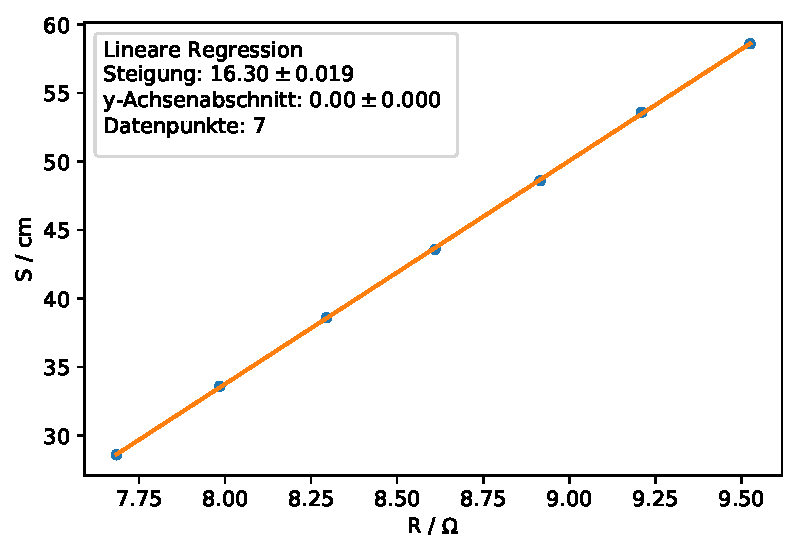
\includegraphics[scale=1]{Bilder/Abstandskal_LinReg.pdf}
	\end{subfigure}
	\begin{subfigure}[]{\textwidth}
	\centering
	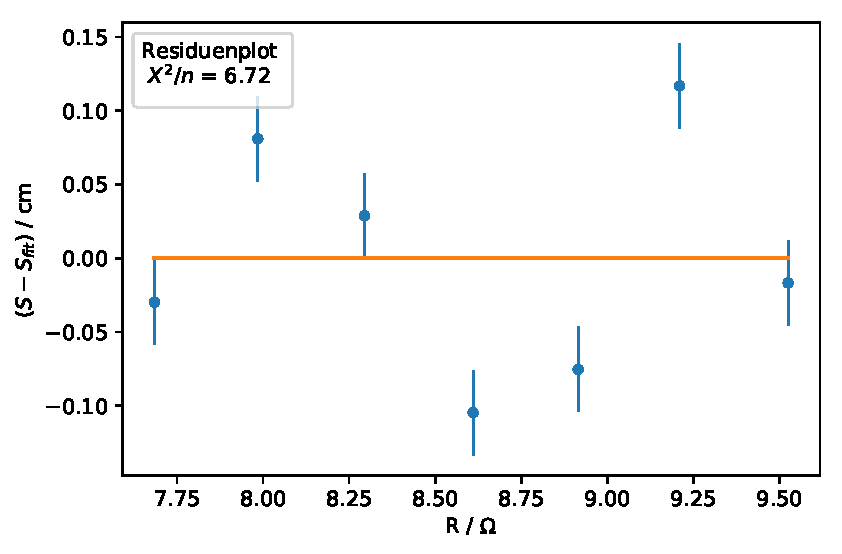
\includegraphics[scale=1]{Bilder/Abstandskal_Residuen.pdf}
	\end{subfigure}
\caption{Lineare Regression der Abstandskalibrierung mit Residuenplot}
\label{Abstandskal_LinReg}
\end{figure}
\end{comment}
\begin{figure}
	\centering
	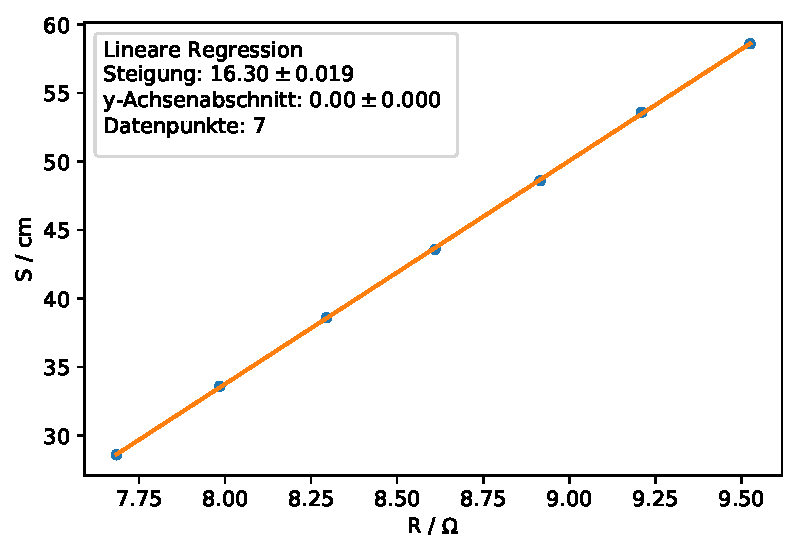
\includegraphics[scale=1]{Bilder/Abstandskal_LinReg.pdf}
	\caption{Lineare Regression der Abstandskalibrierung}
	\label{Abstandskal_LinReg}
\end{figure}
\begin{figure}
	\centering
	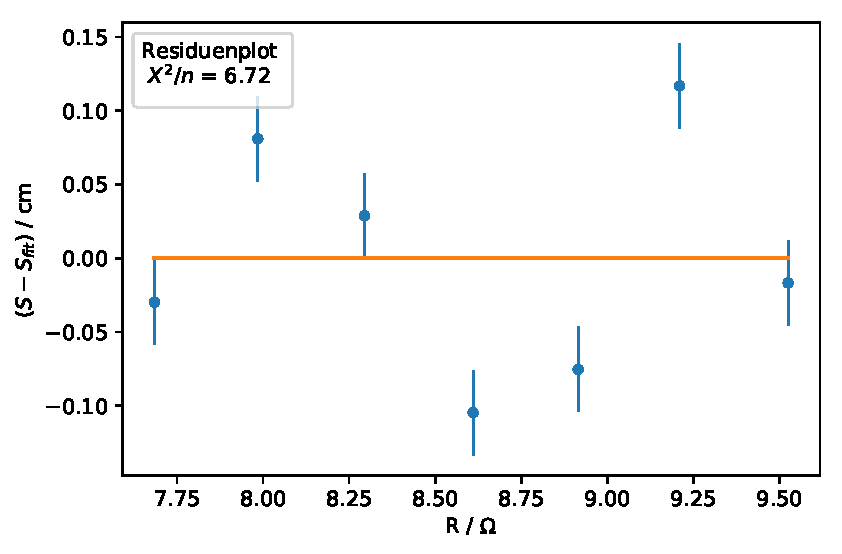
\includegraphics[scale=1]{Bilder/Abstandskal_Residuen.pdf}
	\caption{Residuenplot der Abstandskalibrierung}
	\label{Abstandskal_Residuenplot}
\end{figure}
\\Abb.~\ref{Abstandskal_LinReg} zeigt das Ergebnis der linearen Regression:
\begin{align}
k = 16.30\pm0.019\frac{\text{cm}}{\Omega}
\end{align}
\begin{align}
\frac{\chi^2}{n}=6.72
\end{align}
Der Wert f"ur $\chi^2/n$ ist mit 6.72 sehr gro\ss\ -  ein Zeichen daf"ur, dass unsere Fehlerabsch"atzung zu klein ist. Schwer zu quantisierbare Fehlerquellen, die nicht mit in die Auswertung eingeflossen sind, waren unter anderem, dass der Faden des Wegaufnehmers m"oglicherweise nicht ganz parallel zur Schiene stand und durch das ruckelige Fortbewegen des Empf"angerschlittens teilweise an der Rolle verrutscht. Die Bedeutung des $\chi^2/n$ wird dadurch abgeschw"acht, dass nur 7 Messpunkte in den Fit einflie\ss en. Der Residuenplot zeigt keine Au\ss ergew"ohnlichkeiten, au\ss er der Tatsache, dass die Fehlerbalken nur selten die Nulllinie schneiden, wie bei einem gro\ss en $\chi^2/n$ zu erwarten ist.
\newpage




\section{Abstandsmessung}
\subsection{Versuchsbeschreibung}
Für die späteren Versuche benötigen wir die Abhängigkeit der Intensität von der gemessenen Spannung am Empf"anger.
Dabei wird ausgenutzt, dass die Intensität einer Kugelwelle mit $I\sim\frac{1}{r^2}$ abnimmt. Bei dem Versuch nutzen wir eine Tunneldiode als Empf"anger, die das Signal quadratisch weiterleitet, also
\begin{equation}\label{eq:Spannungvsr}
U\sim E^{-a}\sim\frac{1}{r^{-a}}=r^a,
\end{equation}
mit Erwartung $a=-2$. Die Intensit"at h"angt quadratisch von dem E-Feld ab $I\sim E^2$ und somit 
\begin{equation}
I \sim U^{\frac{2}{-a}}.
\end{equation}
Durch die Messung der Signalspannung $U$ in Abhängigkeit des Abstands $r$ (Gl.~\eqref{eq:Spannungvsr}) zwischen Sender und Empfänger wird in diesem Versuch nun der Parameter $a$ bestimmt.
\subsection{Versuchsaufbau und Durchführung}
Wie bei der Abstandskalibrierung wird der Schlitten, auf dem nun der Empfänger montiert ist, auf der Schiene verschoben. Dabei beginnen wir nahe am Sender und führen eine automatische Messung mit CASSYLab durch, indem wir den Empfänger langsam und gleichmäßig von dem Sender entfernen. Um nun $a$ zu bestimmen, tragen wir $U$ gegen $S$ doppellogarithmisch auf:
\begin{align*}
log(U)=b-a\cdot log(S),
\end{align*}
Die Strecke $S$ entspricht hier dem Radius der Kugelwelle $r$ und wird wieder "uber den Widerstand des Wegaufnehmers gemessen, wobei diesmal eine Schnellkalibrierung "uber zwei Referenzpunkte in CASSYlab vorgenommen wurde. 
\subsection{Versuchsauswertung}
\begin{figure}[H]
\centering
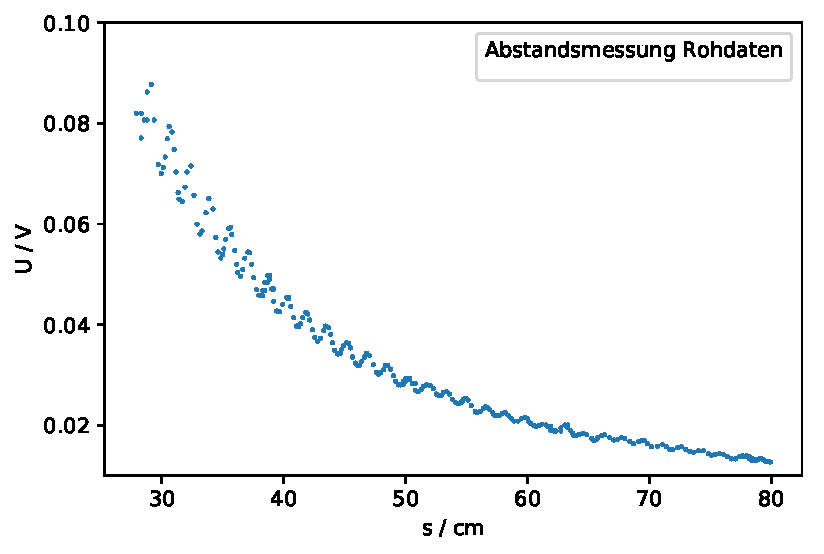
\includegraphics[scale=1]{Bilder/Abstandsabh_Rohdaten.pdf}
\caption{Gemessene Spannung als Funktion des Abstandes zwischen Sender und Empf"anger}
\end{figure}
Wir analysieren die Messwerte, indem wir Weg und Spannung doppellogarithmisch auftragen und eine linearen Regression vornehmen. Der Parameter $a$ ergibt sich nun aus der Steigung. Es wurden folgende Unsicherheiten auf die Messwerte angenommen
\begin{align}
\sigma_S &= \frac{0.5\text{cm}}{\sqrt{12}} \\
\sigma_U &= 0.002\,\text{V}.
\end{align}
Die recht gro\ss e Unsicherheit auf die Strecke ergibt sich dadurch, dass sich die genaue Position des Senders und des Empf"angers innerhalb der Hornantennen nicht genau bestimmen lässt. Au\ss erdem ist die Schnellkalibrierung durch CASSYlab fehleranf"allig, weil nur zwei Messwerte verwendet werden. Wir sch"atzen unsere Messskala deshalb mit einer kleinsten Skalenbreite von 0.5cm ab und nehmen eine Gleichverteilung innerhalb dieser an.\\
Bei Betrachtung der Rohdaten stellen wir fest, dass die Mikrowellen anscheinend an umliegenden Gegenst"anden, Personen oder Raumwämden reflektiert wurden und sich stehende Wellen ausbilden. Die Knoten und Bäuche der stehenden Welle sind im Spannungsverlauf deutlich zu erkennen. Um die Messwerte trotzdem linear annähern zu können, schätzen wir den Fehler auf die Spannung auf ca. 1/3 der durchschnittlichen Spannungsdifferenz zwischen nebeneinanderliegenden Knoten und Bäuchen ab, was einen Wert von $0.002\,\text{V}$ ergibt. Dieser Fehler ist deutlich größer als der Digitalisierungsfehler des CASSY-Geräts von $\frac{0.6 kV}{4096\cdot\sqrt{12}}$, sodass letzteres vernachlässigt wird.
Für die Fehler auf den Logarithmus nutzen wir Gaußsche Fehlerfortpflanzung:
\begin{align}
\sigma(\log(S))&=\frac{\sigma_S}{S}\\
\sigma(\log(U))&=\frac{\sigma_U}{U}
\end{align}
\begin{figure}
	\centering
	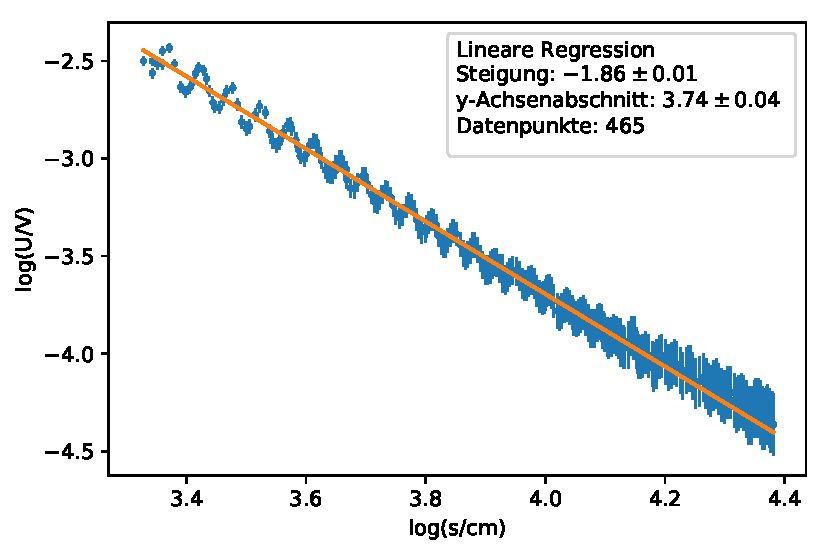
\includegraphics[scale=1]{Bilder/Abstandsabh_LinReg.pdf}
	\caption{Lineare Regression der Abstandsmessung}
	\label{Abstandsabh_LinReg}
\end{figure}
\begin{figure}
	\centering
	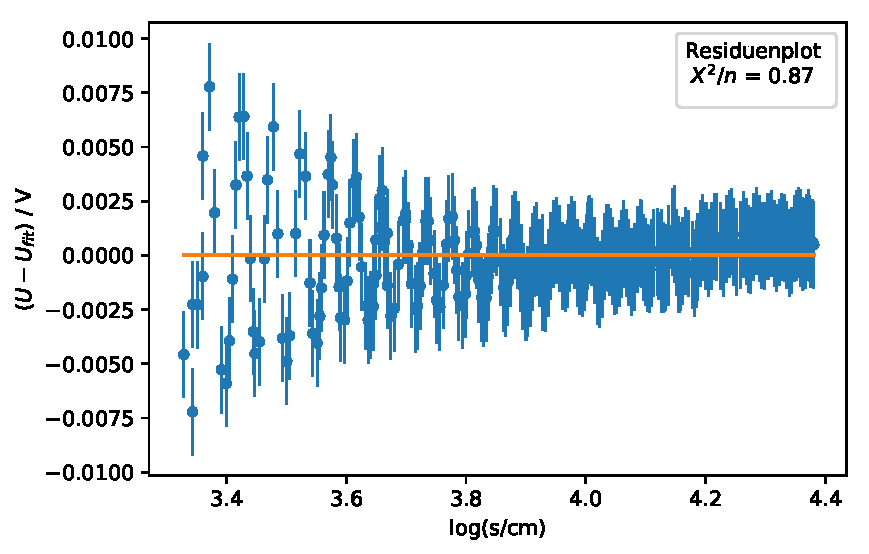
\includegraphics[scale=1]{Bilder/Abstandsabh_Residuen.pdf}
	\caption{Residuenplot der Abstandsmessung}
	\label{Abstandsabh_Residuenplot}
\end{figure}
Abb.~\ref{Abstandsabh_LinReg} stellt die Ergebnisse der Linearen Regression dar. Die Messdaten werden insgesamt gut durch die genäherte Gerade beschrieben und der Residuenplot zeigt keine Auffälligkeiten. Das $\chi^2/n$ ist nur geringfügig kleiner als 1. Wir erhalten einen Wert $a=-1.86$, was etwas kleiner ist als der erwartete Wert von $a=-2$. Ein Grund könnte sein, dass die Tunneldiode das Signal nicht quadratisch umsetzt. Außerdem sendet die Hornantenne keine idealen Kugelwellen aus und die gemessene Spannung wird durch die Reflexion an umliegenden Gegenst"anden verstärkt.
\newpage
\vphantom{v}
\newpage
\section{Stehende Welle}
\subsection{Versuchsbeschreibung}

Mit  Hilfe einer Reflexionswand gegenüber des Senders wird eine stehende Welle erzeugt. Einfallende und reflektierte Welle überlagern sich und ergeben eine stehende Welle, bei der die räumlichen und zeitlichen Oszillationen entkoppelt sind. Es entstehen Knoten in Abständen einer halben Wellenlänge, bei der die Intensität der Welle immer ann"ahernd null ist. Dazwischen liegen Bäuche, die im zeitlichen Mittel eine positive Intensität liefern. In diesem Versuch wird der Empfänger zwischen Sender und Reflexionswand verschoben und die Spannung gegen den Ort aufgezeichnet. Anhand der gemessenen Maxima, die einem Bauch entsprechen, kann die Wellenlänge bestimmt werden: Zwischen $n$ Bäuchen liegen $n/2$ Wellenlängen (Z"ahlung bei null beginnend).
\subsection{Versuchsaufbau und Durchführung}
Für die Vermessung der stehenden Welle wird ein Polarisationsfilter als Reflexionswand verwendet. Dazu wird dessen Polarisationsebene um $90^{\circ}$ zum Sender gedreht. Der Empfänger  befindet sich auf der Schiene zwischen Sender und Reflexionswand, wobei die Hornantenne auf den Polarisationsfilter gerichtet ist.
Der Empfänger wird für die Messung nah beim Polarisationsfilter beginnend in Richtung Sender langsam verschoben. Die Verschiebung wird durch den Wegaufnehmer als Widerstand aufgezeichnet. Mithilfe der Abstandskalibrierung aus dem ersten Versuchsteil kann der Widerstand in eine Strecke umgerechnet werden.
\subsection{Versuchsauswertung}
Abb.~\ref{stehendeWelle} stellt die gemessene Spannung als Funktion des Widerstandes des Wegaufnehmers dar. Wie erwartet sind viele Knoten in Form von Minima und B"auche in Form von Maxima zu erkennen. Von ausgewählten Peaks wurde mit dem Programm CASSYlab der Peakschwerpunkt und die darauf liegende Unsicherheit berechnet, siehe Tabelle \ref{tab:stehendeWellePeaks}.
\begin{table}[H]
	\centering
	\begin{tabular}{|c|c|}
		\hline 
		i&$R_i\pm\sigma_{R_i}$ in k$\Omega$\\ 
		\hline
		0&$5.904\pm0.008$\\
		4&$6.313\pm0.015$\\
		8&$6.713\pm0.016$\\
		14&$7.298\pm0.018$\\
		19&$7.802\pm0.016$\\
		25&$8.398\pm0.021$\\
		29&$8.797\pm0.011$\\
		33&$9.187\pm0.015$\\
		\hline
	\end{tabular} 
	\caption{Positionen der Peaks und ihre Unsicherheit}
	\label{tab:stehendeWellePeaks}
\end{table}
Aus den Messdaten bestimmen wir die Wellenl"ange auf zwei unterschiedliche Arten.\\
Zum einen wird der Abstand $\Delta R=R_{33}-R_0$ zwischen dem Peak bei $R_0=5.90\,\text{k}\Omega$ und dem Peak bei $R_{33}=9.19\,\text{k}\Omega$ berechnet, die Anzahl $n$ dazwischen liegender B"auche gez"ahlt und daraus die Wellenl"ange mit 
\begin{equation}
\lambda=\frac{2k\Delta R}{n}
\end{equation}
berechnet, wobei k der Umrechnungsfaktor aus der Wegkalibrierung ist.  Mit $n=33$ ergibt sich eine Wellenl"ange von $\lambda_1=3.243\,\text{cm}$. Die statstische Unsicherheit wird mit der Gaußschen Fehlfortpflanzung berechnet:
\begin{equation}
\sigma_{\lambda,\text{stat}}=\frac{2k}{33}\sqrt{\sigma_{R_0}^2+\sigma_{R_{33}}^2}=0.017\,\text{cm}
\end{equation}
Dazu kommt ein systematischer Fehler durch den Umrechnungsfaktor k, der auf folgende Weise abgesch"atzt wird:
\begin{align}
\sigma_{\lambda,\text{sys}}=\lambda(k+\sigma_k)-\lambda(k)=\frac{2\Delta R}{33}\sigma_k=0.004\,\text{cm}
\end{align}
Insgesamt erh"alt man so
\begin{equation}
\lambda_1=3.243\pm0.017\pm0.004\,\text{cm}.
\end{equation}
\begin{figure}
\centering
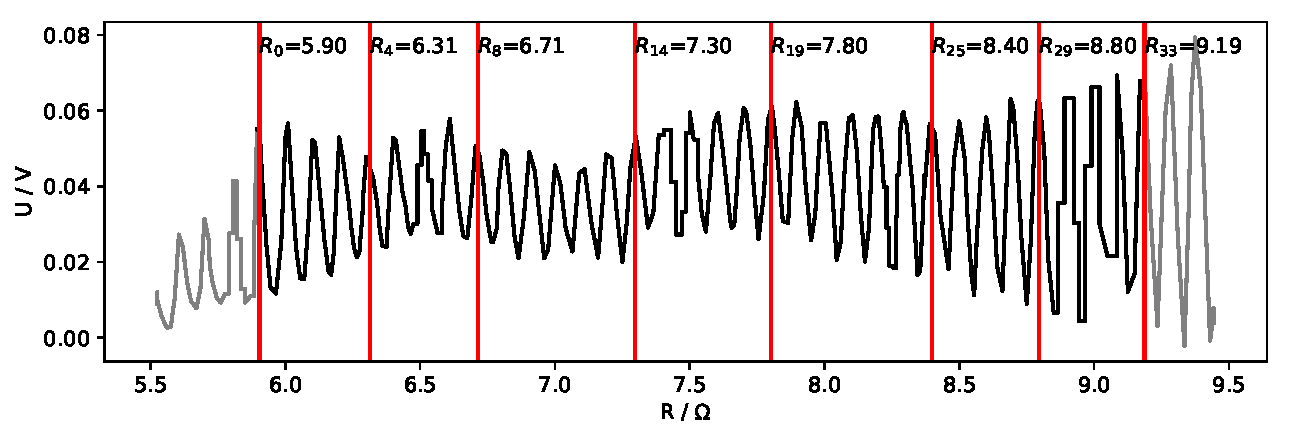
\includegraphics[scale=0.8]{Bilder/stehendeWelle.pdf}
\caption{Gemessene Spannung am Empf"anger als Funktion des Widerstandes des Wegaufnehmers und Markierung ausgew"ahlter Maxima}
\label{stehendeWelle}
\end{figure}Als zweite Methode zur Berechnung der Wellenlänge werden die Positionen der Widerstandspeaks gegen die Nummerierung der Peaks aufgetragen und wir führen eine lineare Regression (Abb.~\ref{stehendeWelle_LinReg}) durch. Die Wellenlänge berechnet sich aus der Steigung $m_{\text{sw}}$ durch
\begin{equation}
\lambda=2km_{\text{sw}}.
\end{equation}
Die Auswertung der linearen Regression ergibt ein $\chi^2/n$ von 0.17. Dieser Wert deutet an, dass die Unsicherheiten auf die Widerstandspeaks kleiner gewählt werden können. Die Steigung $m_{\text{sw}}=0.0996\pm0.0004$ hat nur eine sehr kleine Unsicherheit, was dafür spricht, dass diese Methode zur Wellenlängenbestimmung zuverlässig ist. Der Residuenplot in Abb.~\ref{stehendeWelle_Residuenplot} zeigt, dass die Messwerte gleichmäßig um die genäherte Gerade liegen.
Die Wellenlänge ergibt sich zu $3.246\,\text{cm}$ mit Unsicherheiten
\begin{align}
\sigma_{\lambda,\text{stat}}&=2k\sigma_{m_{\text{sw}}}=0.013\,\text{cm}\\
\sigma_{\lambda,\text{sys}}&=2m_{\text{sw}}\sigma_k=0.004\,\text{cm}
\end{align}
Insgesamt also
\begin{equation}
\lambda_2=3.246\pm0.017\pm0.004\,\text{cm}.
\end{equation}
Die Wellenlängen $\lambda_1$ und $\lambda_2$ liegen nah beieinander und überschneiden sich im Rahmen ihrer Unsicherheiten. Allerdings ist bei der Betrachtung zu berücksichtigen, dass sich die beiden vorgestellten Methoden in ihrer Herangehensweise ähneln und die beiden Werte der Wellenlänge voneinander abh"angen.
\begin{figure}
	\centering
	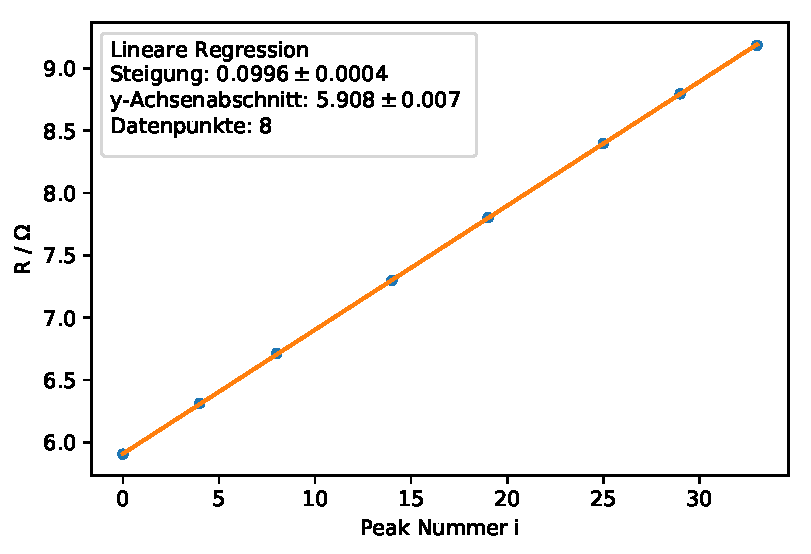
\includegraphics[scale=1]{Bilder/stehendeWelle_LinReg.pdf}
	\caption{Lineare Regression der Spannungspeaks der stehenden Welle}
	\label{stehendeWelle_LinReg}
\end{figure}
\begin{figure}
	\centering
	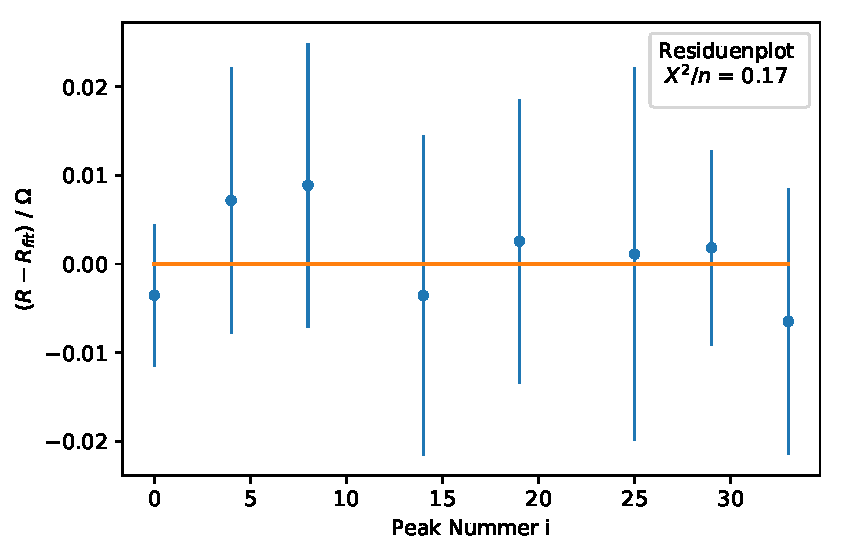
\includegraphics[scale=1]{Bilder/stehendeWelle_Residuen.pdf}
	\caption{Residuenplot}
	\label{stehendeWelle_Residuenplot}
\end{figure}

\newpage
\section{Polarisationsfilter}
\subsection{Versuchsbeschreibung}
In diesem Versuch wird das Gesetz von Malus veranschaulicht. Dieses besagt, dass linear polarisierte Wellen beim Passieren eines Polarisationsfilters ihre Schwingungsebene drehen und sich die Intesität auf
\begin{equation}
I=I_0\cos^2{\phi}
\end{equation}
verringert, wobei $\phi$ der Winkel zwischen einfallender Polarisationsebene und Ausrichtung des Polarisators ist. In unserem Versuch werden Sender und Empf"anger mit paralleler Ausrichtung der Dipole positioniert. Dazwischen befindet sich ein Polarisationsfilter mit drehbarer Polarisationsrichtung $\phi$. Wir bestimmen die Intensit"at am Empf"anger als Funktion von $\phi$ und erwarten eine Abh"angigkeit
\begin{equation}\label{eq:MalusGesetzx}
I=I_0\cos^x{\phi}
\end{equation}
mit $x=4$, weil der Empf"anger als Analysator ebenfalls polarisierend wirkt.
\subsection{Versuchsaufbau und Durchführung}
Die Hornantennen werden mit einem Abstand von ca. 40cm und zueinander ausgerichtet auf der Schiene befestigt. Dazwischen wird der Polarisationsfilter montiert, ein Gitter aus elektrisch leitenden St"aben. Die Polarisationsrichtung l"asst sich manuell um $\ang{360}$ drehen, wobei die minimale Skalenbreite bei $\ang{1}$ liegt. Nun wird die Polarisationsrichtung in Abst"anden von $\ang{10}$ manuell verschoben, angefangen bei maximaler Ausl"oschung bei $\phi=-\ang{90}$ bis zum Winkel $\phi=\ang{270}$, wobei nach jeder Drehung des Filters das Signal des Empf"angers als Spannung aufgezeichnet wird.
\subsection{Versuchsauswertung}
Abb.~\ref{Polarisation_Rohdaten} stellt den gemessenen Spannungsverlauf am Empf"anger als Funktion der Polarisationsrichtung $\phi$ dar. Wie erwartet ist die Spannung und somit Intensit"at bei $\ang{0}$ und bei $\ang{180}$ maximal; bei $\ang{-90}$, $\ang{90}$ und $\ang{270}$ ist die Spannung dagegen nahezu bei 0. Die Werte liegen symmetrisch um $\ang{90}$ und somit ist keine weitere Anpassung der Gradskala notwendig.
\begin{figure}
\centering
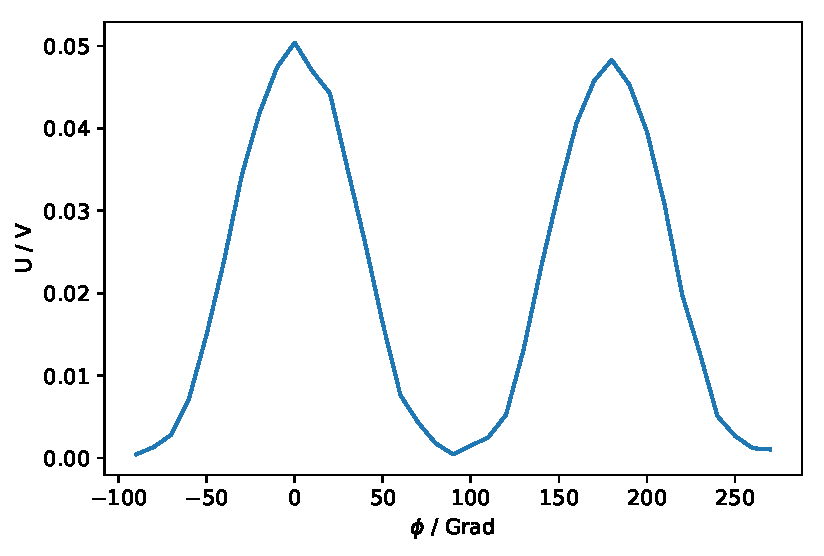
\includegraphics[scale=1]{Bilder/Polarisation_Rohdaten.pdf}
\caption{Spannungsverlauf in Abh"angigkeit der Ausrichtung des Polarisationsfilters}
\label{Polarisation_Rohdaten}
\end{figure}
\begin{figure}
	\centering
	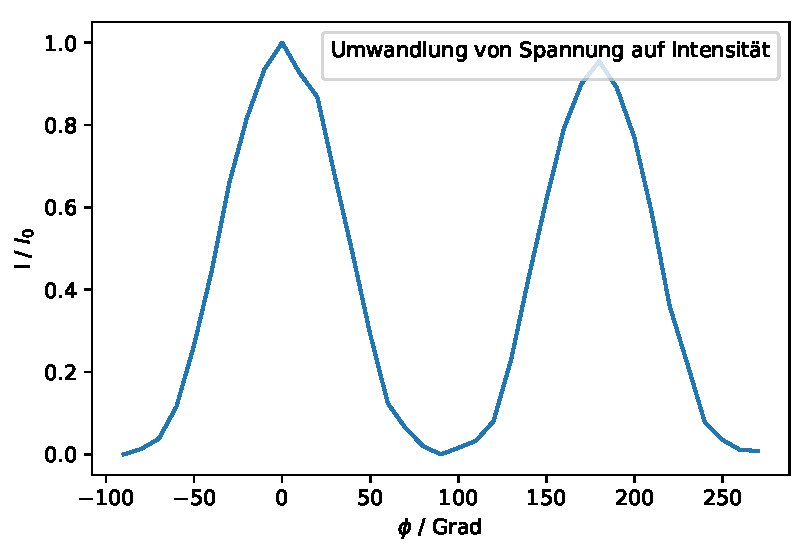
\includegraphics[scale=1]{Bilder/Polarisation_Intensitaet.pdf}
	\caption{Intensität Polarisation}
	\label{Polarisation_Intensitaet}
\end{figure}
Um den Faktor $x$ aus Gl.~\eqref{eq:MalusGesetzx} zu erhalten, wird zun"achst die Spannung mit $I=(U-U_0)^{-2/a}$ in die Intensit"at umgerechnet, wobei $U_0$ der kleinste gemessene Wert der Spannung ist (Abb.~\ref{Polarisation_Intensitaet}). Anschließend tragen wir $\log{I/I_0}$ gegen $\log{|cos{\phi}|}$ auf, wobei $I_0$ der größte erhaltene Wert von $I$ in unserer Berechnung ist, und f"uhren eine lineare Regression durch. Die Steigung entspricht dem gesuchten Wert f"ur $x$. Damit die logarithmischen Werte und die f"ur die Regression ben"otigten Unsicherheiten endliche Werte ergeben, werden die Punkte mit $\phi=\{\ang{-90},\ang{0},\ang{90},\ang{180},\ang{270}\}$ nicht in die Berechnung mit einbezogen.\\
Die Unsicherheiten auf die Messgr"o\ss en werden folgendermaßen abgeschätzt:
\begin{align*}
\sigma_\phi &= \frac{\ang{1}}{\sqrt{12}} \\
\sigma_U &= 0.0005\,\text{k}\Omega\\
\end{align*}
Wie Wahl f"ur $\sigma_{\phi}$ beruht auf der Annahme, dass die Messwerte innerhalb der kleinsten Skalenbreite gleichverteilt sind. Der Fehler auf $U$ ergibt sich aus den Schwankungen der Spannungswerte im station"aren Zustand, wie aus unserem Messungen herauszulesen ist. Dieser ist um eine Gr"o\ss enordnung größer als der Digitalisierungsfehler des CASSY Sensors.
Die Fehler auf $\log{I/I_0}$ und $\log{|cos{\phi}|}$ werden durch Fehlerfortpflanzung berechnet. Eigentlich m"usste die systematische Unsicherheit auf $a$ getrennt betrachtet werden. Weil die f"ur das Praktikum zur Verf"ugung stehenden Python-Funktionen f"ur die lineare Regression keine Trennung von statistischen und systematischen Fehlern vorsieht, nehmen wir vereinfachend an, $\sigma_a$ sei ein statistischer Fehler und nehmen ihn bei der Gaußschen Fehlerfortpflanzung mit auf. Damit ergibt sich
\begin{align}
\log{\frac{I}{I_0}}=-\frac{2}{a}\log(U-U_0)&-\log(I_0)\\
\Rightarrow\sigma(\log{\frac{I}{I_0}})&=\sqrt{\left(\frac{2\sigma_a}{a^2}\log(U-U_0)\right)^2+\left(\frac{2\sigma_U}{a(U-U_0)}\right)^2}\\
\sigma(\log|\cos{\phi}|)&=\Big|\frac{sin{\phi}}{\cos{\phi}}\Big|\sigma_{\phi}
\end{align} 
Die lineare Regression ist in Abb.~\ref{Polarisation_LinReg} dargestellt und gibt einen Wert f"ur $x$ von $x=2.99\pm0.04$. Somit ist der gemessene Wert deutlich kleiner als die Erwartung $x=4$. Das $\chi^2/n$ ist mit 5.12 zu gro\ss, ein Zeichen dafür, dass unsere Fehler zu klein gewählt wurden oder die Messdaten nicht gut durch eine Gerade dargestellt werden. Letzere Vermutung wird dadurch bekräftigt, dass f"ur kleine Werte von $|\cos{\phi}|$ die Ausgleichsgerade der linearen Regression deutlich unterhalb der gemessenen Werte liegt, wie im Residuenplot in Abb.~\ref{Polarisation_Residuenplot} zu erkennen. Nicht berücksichtigte Fehlerquellen sind wieder die Reflexion der Wellen an umliegenden Gegenständen und ein fehlerbehafteter Polaristionsfilter, der möglicherweise auch die Intensität der Mikrowellen abschwächt, wenn die Gitterstäbe senkrecht zur Dipolausrichtung stehen. 

\begin{figure}
	\centering
	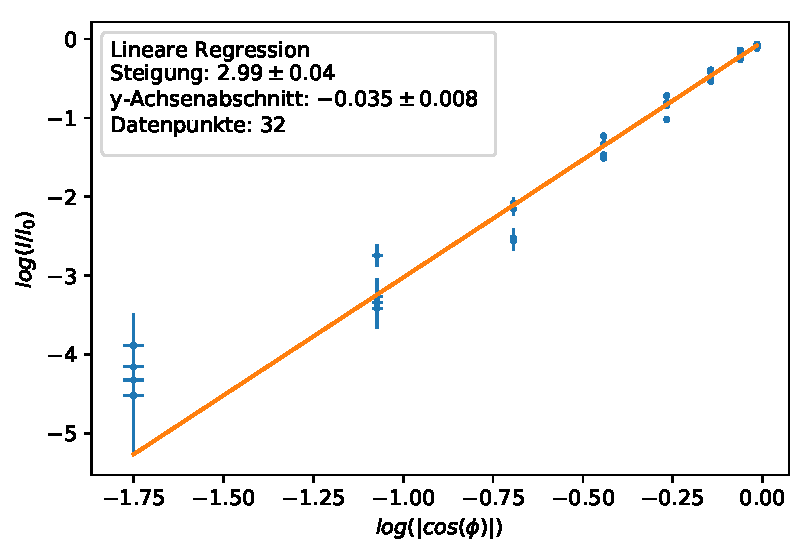
\includegraphics[scale=1]{Bilder/Polarisation_LinReg.pdf}
	\caption{Lineare Regression zum Gesetz von Malus}
	\label{Polarisation_LinReg}
\end{figure}
\begin{figure}
	\centering
	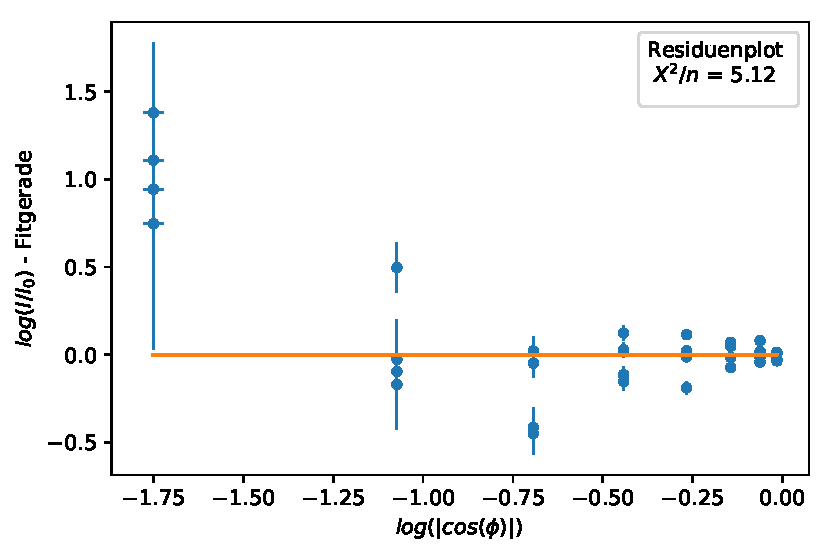
\includegraphics[scale=1]{Bilder/Polarisation_Residuen.pdf}
	\caption{Residuenplot zum Gesetz von Malus}
	\label{Polarisation_Residuenplot}
\end{figure}


\newpage
\vphantom{v}
\newpage
\section{Winkelkalibrierung}
\subsection{Versuchsbeschreibung}
In diesem Vorversuch wird der Winkelaufnehmer am Drehtisch kalibriert, um in den folgenden Versuchen den gemessenen Widerstand in einen Winkel umrechnen zu k"onnen. Die Vorgehensweise ist analog zur Kalibrierung des Wegaufnehmers.
\subsection{Versuchsbeschreibung, Aufbau und Durchführung} 
Bei den Versuchen zur Brechung und zur Frustrierten Totalen Internen Reflexion (FTIR) wird der Empfänger an den Schwenkarm des motorbetriebenen Drehtisches befestigt. Die Reflexionswand wird abgebaut. Die Hornantenne befindet sich auf einem Radius von etwa 30cm und auf gleicher Höhe wie der Sender. Ähnlich wie beim Wegaufnehmer erfolgt die Winkelmessung mit einem Drehpotentiometer, der am Drehtisch verbaut ist und einen Widerstand in Abhängigkeit des Dreharmwinkels ausgibt. Dieser Winkelaufnehmer wird in diesem Vorversuch kalibriert. Dazu werden die am Drehtisch manuell abgelesenen Winkel $\gamma$ in äquidistanten Schritten von $\ang{10}$ im Messwertbereich von $\ang{-90}$ bis $\ang{90}$ gegen den Widerstand aufgetragen. Wie bereits in Tabelle \ref{tab:MessparameterAllgemein} zusammengefasst, werden die Widerstandswerte über 200ms gemittelt und der Messbereich des Winkelaufnehmers auf 0..10k$\Omega$ gesetzt. Die Skalenbreite zur Winkelablesung am Drehtisch beträgt $\ang{5}$.
\subsection{Versuchsauswertung}
Die gemessenen Winkel $\gamma$ werden in Abb.~\ref{Winkelkalibrierung_Rohdaten} gegen den Widerstand des Winkelaufnehmers aufgetragen. "Ahnlich wie bei der Kalibrierung des Wegaufnehmers werden die Winkel und Widerst"ande zun"achst zu ihren Mittelwerten $\bar{\gamma},\bar{R}$ verschobenen, bevor die lineare Regression durchgef"uhrt wird. Der Grund f"ur die Verschiebung ist, dass die Korrelation zwischen Steigung und y-Achsenabschnitt minimiert wird.
\begin{align}\label{eq:Winkelkal}
\gamma-\bar{\gamma}=k_{\gamma}\cdot (R-\bar{R}) + b_{\gamma}
\end{align}
F"ur die Unsicherheit auf den Widerstand wird der Digitalisierungsfehler des CASSY Sensors angenommen:
\begin{equation}
\sigma_R=\frac{10\text{k}\Omega}{4096\cdot\sqrt{12}}
\end{equation}
Der Fehler auf $\gamma$ wird mit der kleinsten Skalenbreite abgesch"atzt unter Annahme einer Gleichverteilung:
\begin{equation}
\sigma_{\gamma}=\frac{\ang{5}}{\sqrt{12}}
\end{equation}
Die lineare Regression erzeugt eine Ausgleichsgerade mit Steigung $k_{\gamma}=-0.68\pm0.05$. Der y-Achsenabschnitt $b_{\gamma}$ ist null aufgrund der Verschiebung der Messwerte zu ihren Mittelwerten. Das $\chi^2/n$ ist mit 0.03 sehr klein, was darauf hinweist, dass die Unsicherheiten zu gro\ss \ gew"ahlt wurden. Diese Vermutung best"atigt sich im Residuenplot (Abb.~\ref{Winkelkal_Residuenplot}), wo zu erkennen ist, dass die Fehlerbalken aller Messpunkte die Regressionsgerade schneiden. Vor allem der Fehler auf $\gamma$ wird in Realit"at kleiner sein als in der linearen Regression angenommen, weil sich die Winkel trotz fehlender Skalenstriche deutlich genauer am Drehteller ablesen lassen.\\
Der Fehler auf $k_{\gamma}$ wird in den Folgeversuchen als systematischer angenommen, weil er einen zus"atzlichen Beitrag als Skalenfehler bei der Umrechnung vom Widerstand auf den Winkel liefert.
\begin{figure}
\centering
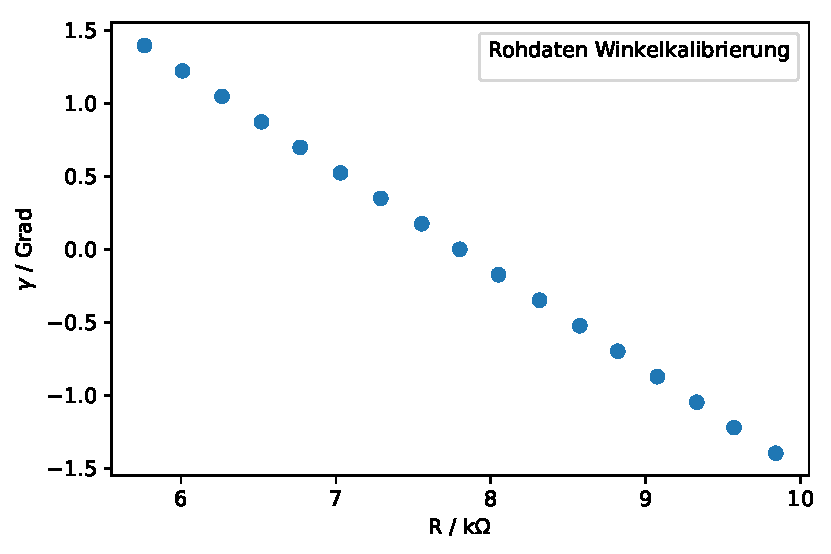
\includegraphics[scale=1]{Bilder/Winkelkal_Rohdaten.pdf}
\caption{Gemessene Winkel $\gamma$ am Drehtisch als Funktion des Widerstandes des Winkelaufnehmers}
\label{Winkelkalibrierung_Rohdaten}
\end{figure}

\begin{figure}
\centering
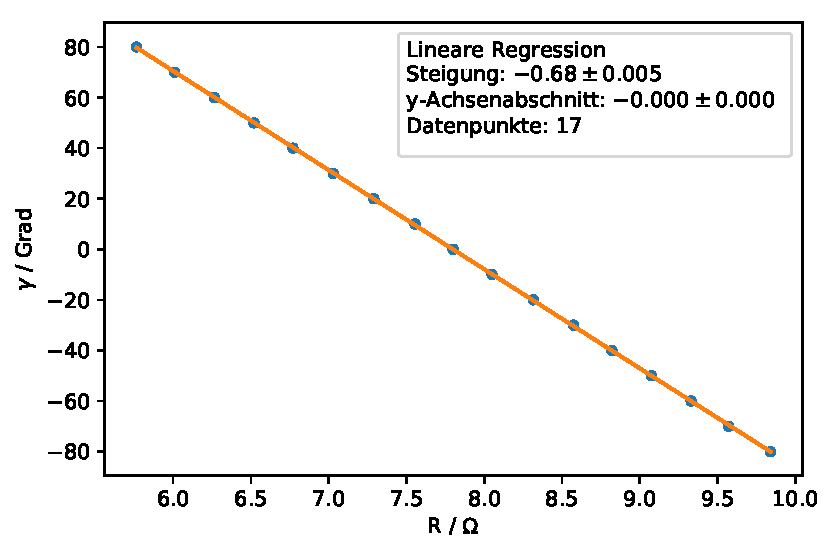
\includegraphics[scale=1]{Bilder/Winkelkal_LinReg.pdf}
\caption{Lineare Regression der Winkelkalibrierung}
\label{Winkelkal_LinReg}
\end{figure}
\begin{figure}
\centering
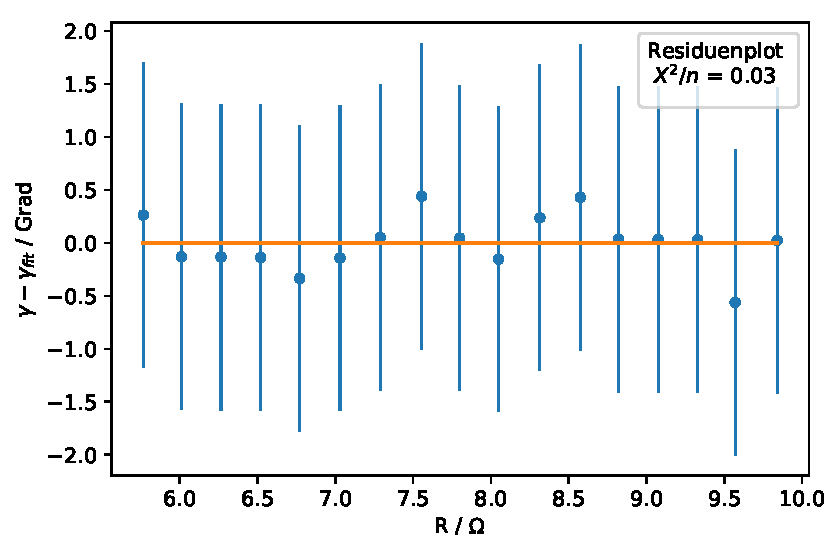
\includegraphics[scale=1]{Bilder/Winkelkal_Residuen.pdf}
\caption{Residuenplot der Winkelkalibrierung}
\label{Winkelkal_Residuenplot}
\end{figure}
\newpage
\vphantom{v}
\newpage

\section{Brechung am PE-Halbzylinder}

\subsection{Versuchsbeschreibung}
In diesem Versuch wird die Brechung der Mikrowellen an der Grenzfläche von PE und Luft untersucht. Das Snelliussche Brechungsgesetz bezieht Einfallswinkel $\alpha$, Brechungswinkel $\beta$ und die Brechungsindexe des Mediums der einfallenden Welle $n_1$ und der transmittierten Wellen $n_2$ aufeinander:
\begin{equation}
n_1\sin{\alpha}=n_2\sin{\beta}
\end{equation}
Durch Variation der Einfallswinkel bei der Brechung an PE-Halbzylindern und das Messen der zugehörigen Ausfallswinkel, lässt sich der Brechungsindex von PE bestimmen. 
\subsection{Versuchsaufbau und Durchführung}
Der Versuchsaufbau entspricht dem der Winkelkalibrierung mit folgenden Ergänzungen: Über dem Drehteller wird horizontal eine runde Platte mit Winkelskala montiert, die mittels eines U-Profils am Schienenkreuz befestigt ist. Somit bewegt sie sich nicht mit dem Schwenkarm des Drehtellers mit. Auf dieser Platte werden PE-Halbzylinder gelegt, sodass sich unterschiedliche Einfallswinkel ergeben, wenn die Mikrowellen vom Sender auf den Halbzylinder treffen. Je nachdem, ob die runde Seite des Halbzylinders auf den Empfänger oder auf den Sender zeigt, findet die Brechung von PE in Luft oder von Luft in PE statt. Der Schwenkarm dreht sich während der Messung im Halbkreis um den Drehtisch und das CASSY-Gerät zeichnet die verstärkte Spannung am Empfänger gegen den Widerstand des Winkelaufnehmers auf.\\
Bei der Brechung von Luft in PE nehmen wir die Intensitätsverteilung für die Einfallswinkel $\alpha_1=\{0,\ang{20},\ang{40},\ang{60}\}$ auf, bei der Brechung von PE in Luft wählen wir Einfallswinkel $\alpha_2=\{0,\ang{-20},\ang{-40}\}$. Im Verlauf des Versuches gab unser Winkelaufnehmer immer häufiger Fehlwerte aus, sodass wir den Versuch nach der Messung von $\alpha_2=\ang{-40}$ abbrechen mussten. Die bis dahin aufgenommenen Daten reichen jedoch f"ur eine erste Auswertung aus.
\subsection{Versuchsauswertung}
Die Abb.~\ref{Brechung_Rohdaten} und \ref{Brechung2_Rohdaten} zeigen den Spannungsverlauf des Empf"angers in Abh"angigkeit des Schwenkarmwinkels $\gamma$ f"ur unterschiedliche Einfallswinkel. Abb.~\ref{Brechung_Rohdaten} zeigt die Spannung f"ur die Brechung von Luft nach PE, Abb.~\ref{Brechung2_Rohdaten}  f"ur die Brechung von PE nach Luft. Die Werte von $\gamma$ wurden aus den gemessenen Widerst"anden mit der Winkelkalibrierung des Wegaufnehmers berechnet (Gl.~\eqref{eq:Winkelkal}). Die Peaks der Spannungskurven geben den Winkel von $\gamma$ an, in die die Welle w"ahrend der Brechung transmittiert wird. Diese Werte wurden mit dem Peakschwerpunktfinder in CASSYlab ermittelt und lauten
\begin{align}
\gamma_{10}&=\ang{0.39}\pm\ang{0.15}\\
\gamma_{11}&=\ang{7.95}\pm\ang{0.15}\\
\gamma_{12}&=\ang{16.15}\pm\ang{0.14}\\
\gamma_{13}&=\ang{26.97}\pm\ang{0.14}\\
\gamma_{20}&=\ang{-1.03}\pm\ang{0.06}\\
\gamma_{21}&=\ang{-14.79}\pm\ang{0.08}\\
\gamma_{22}&=\ang{-33.37}\pm\ang{0.34}
\end{align}
Der Ausfallswinkel $\beta$ berechnet sich folgenderma\ss en als Funktion von $\alpha$ und $\gamma$
\begin{align}
\text{Brechung von Luft nach PE: }\beta_1&=\alpha_1-\gamma_1\\
\text{Brechung von PE nach Luft: }\beta_2&=\alpha_2+\gamma_2
\end{align} 
F"ur die Berechnung des Brechungsindexes wird $\sin{\alpha_1}$ gegen $\sin{\beta_1}$ aufgetragen, bzw $\sin{\beta_2}$ gegen $\sin{\alpha_2}$ und es wird jeweils eine lineare Regression durchgef"uhrt. Die Steigungen entsprechen dem Brechungsindex von PE (der Brechungsindex von Luft wird mit 1 angenn"ahert). Die Unsicherheiten auf $\sin{\alpha}$ und $\sin{\beta}$ wurden mit Gau\ss scher Fehlerfortpflanzung berechnet, wobei
\begin{align}
\sigma(\alpha)=\frac{\ang{5}}{\sqrt{12}}\\
\sigma(\beta)=\sqrt{\sigma^2(\alpha)+\sigma^2(\gamma)}
\end{align}
Ersteres wird damit begr"undet, dass die kleinste Skalenbreite der Platte mit den PE-Halbzylindern $\ang{5}$ war.
\begin{figure}
	\centering
	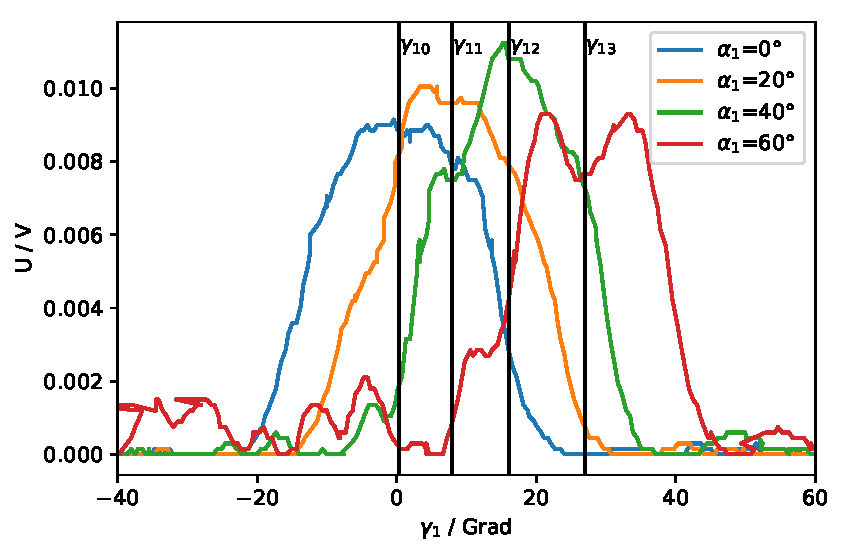
\includegraphics[scale=1]{Bilder/Brechung_gamma.pdf}
	\caption{Winkel $\gamma$ als Funktion der am Empf"anger ausgegeben Spannung f"ur die vier Einfallswinkel $\alpha_1$ bei der Brechung von Luft in PE. Markierung der Spannungspeaks mit schwarzen vertikalen Linien}
	\label{Brechung_Rohdaten}
\end{figure}
\begin{figure}
	\centering
	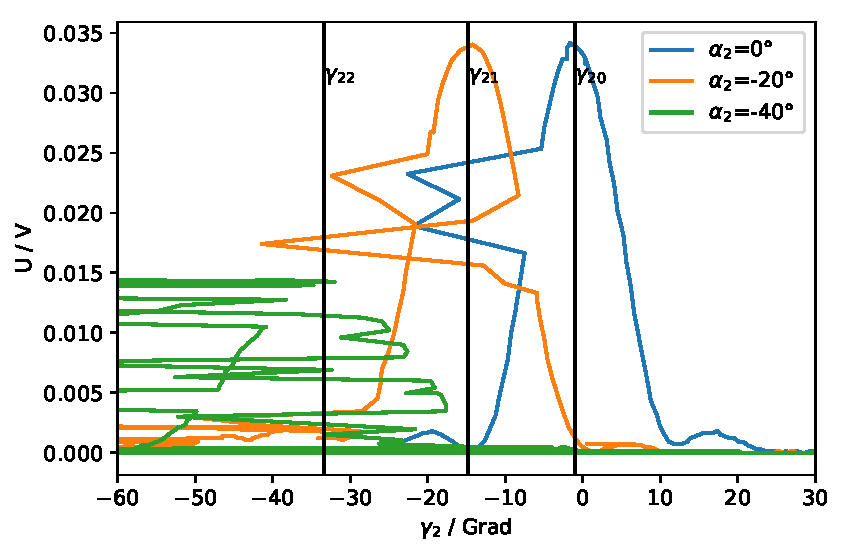
\includegraphics[scale=1]{Bilder/Brechung_gamma2.pdf}
	\caption{Winkel $\gamma$ als Funktion der am Empf"anger ausgegeben Spannung f"ur die drei Einfallswinkel $\alpha_2$ bei der Brechung von PE in Luft. Markierung der Spannungspeaks mit schwarzen vertikalen Linien}
	\label{Brechung2_Rohdaten}
\end{figure}
\begin{figure}
	\centering
	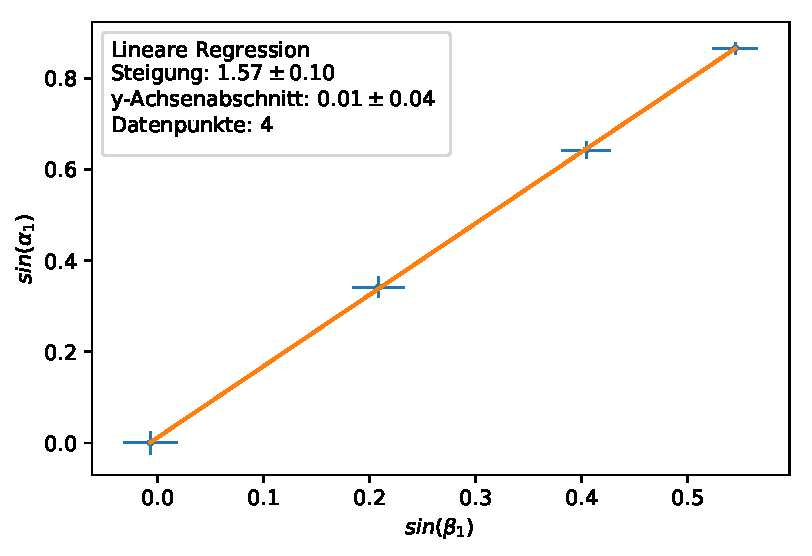
\includegraphics[scale=1]{Bilder/Brechung_LinReg.pdf}
	\caption{Lineare Regression zur Bestimmung des Brechungsindexes bei der Brechung von Luft in PE}
	\label{Brechung_LinReg}
\end{figure}
\begin{figure}
	\centering
	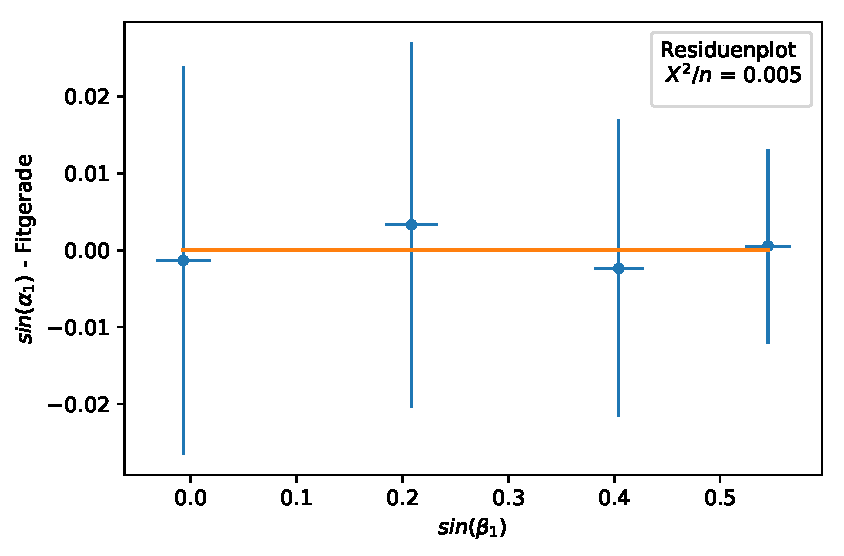
\includegraphics[scale=1]{Bilder/Brechung_Residuen.pdf}
	\caption{Residuenplot zum Versuch zur Brechung von Luft in PE}
	\label{Brechung_Residuenplot}
\end{figure}
\begin{figure}
	\centering
	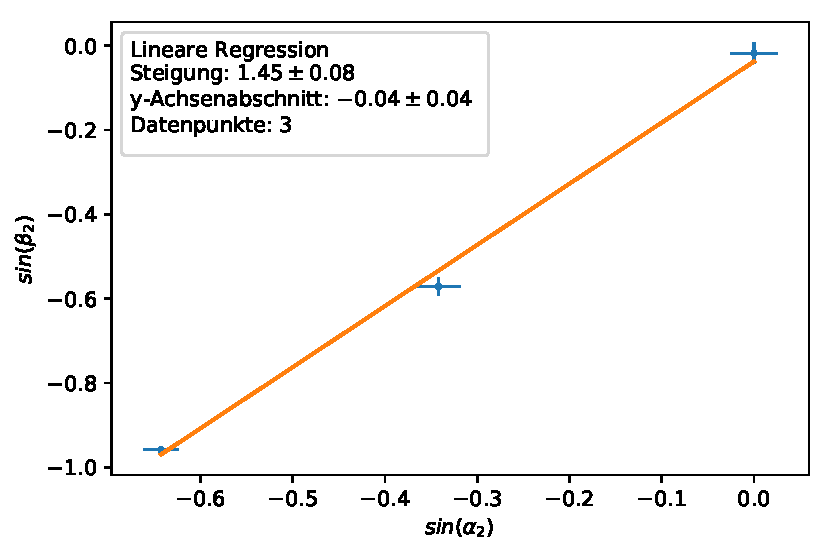
\includegraphics[scale=1]{Bilder/Brechung_LinReg2.pdf}
	\caption{Lineare Regression zur Bestimmung des Brechungsindexes bei der Brechung von PE in Luft}
	\label{Brechung2_LinReg}
\end{figure}
\begin{figure}
	\centering
	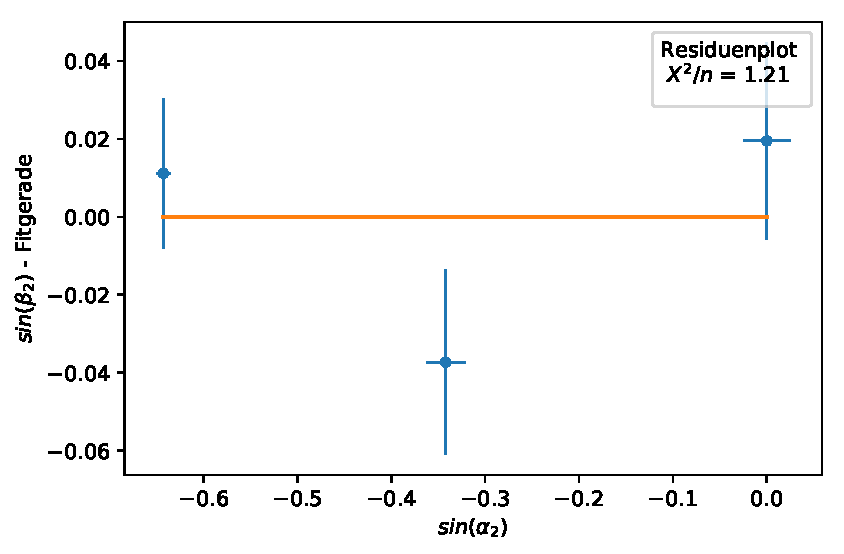
\includegraphics[scale=1]{Bilder/Brechung_Residuen2.pdf}
	\caption{Residuenplot zum Versuch zur Brechung von PE in Luft}
	\label{Brechung2_Residuenplot}
\end{figure}
\\Die Abbildungen \ref{Brechung_LinReg} und \ref{Brechung2_LinReg} stellen die Ergebnisse dar, die Abbildungen \ref{Brechung_Residuenplot} und \ref{Brechung2_Residuenplot} die dazugeh"origen Residuenplots. Das $\chi^2/n$ f"ur die Brechung von Luft in PE ist zu klein, was zeigt, dass unsere Fehler zu groß gew"ahlt wurden. Wie bei der Winkelkalibrierung l"asst sich der Winkel auf $\alpha$ besser einstellen, als die Messskalenbreite vermuten l"asst. Die Residuenplots zeigen keine Auff"alligkeiten, die Messwerte liegen gleichm"a\ss ig um die Ausgleichsgerade. Die Steigung der Regressionsgrade f"ur die Brechung von Luft in PE $n_{\text{PE},1}=1.57\pm0.10$ "uberschneidet sich mit dem Literaturwert von $n_{\text{PE}}=1.55$ (Quelle: Versuchshandbuch) im 1-$\sigma$ Intervall, die Steigung der Regressionsgraden f"ur die Brechung von PE in Luft $n_{\text{PE},2}=1.45\pm0.08$ schneidet den Literaturwert im 2-$\sigma$ Intervall. Somit geben die Messergebnisse sehr gut das Snelliussche Brechungsgesetz wieder.
\newpage
\vphantom{v}
\newpage
\section{Optischer Tunneleffekt}

\subsection{Versuchsbeschreibung}
In diesem Versuch wird eine quantitative Messung zur Frustrierten Totalen Internen Reflexion (FTIR) realisiert. Trifft eine Welle in einem Medium und Brechungsindex $n$ auf einen Spalt mit kleinerem Brechungsindex unter einem Einfallswinkel, der größer ist als der Grenzwinkel der Totalreflexion, wird trotzdem ein Teil der Welle transmittiert, wenn die Spaltbreite $D$ klein gegenüber der Wellenlänge $\lambda$ ist. Die Intensität der transmittierten Welle hängt exponentiell von der Spaltbreite und der Wellenlänge ab:
\begin{equation}
I_T \sim exp(\frac{-2\pi D}{\lambda})
\end{equation}
Dieser Zusammenhang wird in diesem Versuch untersucht, indem die Intensität der transmittierten Welle für unterschiedliche Spaltbreiten gemessen wird.
\subsection{Versuchsaufbau und Durchführung}
Wie im vorherigen Versuch wird der Empfänger auf dem Schwenkarm des Drehtellers befestigt. Zwischen Sender und Empfänger werden auf dem U-Profil zwei Halbzylinder so mit den flachen Seiten aneinander platziert, dass sie einen Vollzylinder mit Spalte der Breite $D$ darstellen. Die Halbzylinder werden so gedreht, dass die vom Sender ausgegebene Welle ungebrochen in das PE eindringt und anschließend mit einem Einfallswinkel von $60^{\circ}$ auf die Luftspalte trifft. Obwohl bei diesem Winkel klassischerweise auschließlich eine Totalreflexion stattfinden sollte, wird nur ein Teil der Welle reflektiert und der andere durch den optischen Tunneleffekt in den zweiten Halbzylinder transmittiert. Wärend der Messung fährt der Empfänger angetrieben durch den Motor des Drehtellers um die beiden Prismen im Winkel von $-80^{\circ}$ bis $80^{\circ}$ und zeichnet die Intensität als Spannung auf. So kann sowohl die transittierte als auch die reflektierte Intensität gemessen werden. Durch Variation der Spaltbreiten $D$ mithilfe von Abstandsblechen lässt sich der Zusammenhang zwischen Spaltbreite und Intensität der transmittierten Welle untersuchen.


\subsection{Versuchsauswertung}
Die erfasste Spannung wird "uber $I\sim U^{-2/a}$  auf Intensit"aten umgerechnet und in Abb.~\ref{FTIR_Rohdaten} aufgetragen. Die drch den Peakschwerpunktfinder des CASSYlabs erhaltenen Maxima lauten
\begin{align}
I'_{T,1mm}&=0.0209\\
I'_{T,4mm}&=0.0095\\
I'_{T,10mm}&=0.0020\\
I_{R,1mm}&=0.0052\\
I_{R,4mm}&=0.0152\\
I_{R,10mm}&=0.0217
\end{align} 
wobei die Werte einheitslos betrachtet werden, weil nur das relative Verhältnis untereinander von Bedeutung ist. Wie erwartet sinkt die maximale Intensit"at der transmittierten Welle bzw steigt die Intensit"at der reflektierten Welle bei größer werdendem Spaltabstand $D$. Da bei der transmittierten Welle Beugungs- und Interferenzerscheinungen auftreten, die die Intensit"at der transmittierten Welle verf"alschen, und dieser Effekt vor allem bei den Spaltbreiten $4\,\text{mm}$ und $10\,\text{mm}$ erkennbar sind, wir die totale Intensit"at $I_{tot}$ bestimmt durch
\begin{equation}
I_{tot}=I_{R,1mm}+I'_{T,1mm}
\end{equation}
Statt der ausgelesenen transmittierten Wellen $I'_{T,i}$ rechnen wir im folgenden mit $I_{T,i}=I_{tot}-I_{R,i}$. Als nächstes werden $D$ und $\log(I-T/I_{tot})$ gegeneinander aufgetragen und eine lineare Regression durchgef"uhrt. Der Fehler auf $D$ wird mit 
\begin{equation}
\sigma_D=\frac{1\,\text{mm}}{\sqrt{12}}
\end{equation}
abgesch"atzt durch Annahme einer Gleichverteilung und einer minimalen Skalenbreite von 1mm der Abstandsbleche. Der Fehler auf $I_R$ und $I_{tot}$ wird abgesch"atzt durch 
\begin{equation}
\sigma_I\equiv\sigma(I_{tot})=\sigma(I_R)=\frac{1}{2}(\max(I_R+I'_T)-\min(I_R+I'_T))
\end{equation}
und durch Fehlerfortpflanzung
\begin{equation}
\sigma({\log(I_T/I_{tot})})=\frac{I_R\sigma_{I}}{I_{tot}-I_R}\sqrt{\frac{1}{I_{tot}^2}+\frac{1}{I_R^2}}
\end{equation}
Der systematische Fehler durch die Umrechnung von Spannung zu Intensit"at wird vernachl"assigt. Die Ergebnisse der linearen Regression sind in Abb.~\ref{FTIR_LinReg} und \ref{FTIR_Residuenplot} dargestellt. Das $\chi^2/n$ ist bei drei Messpunkten wenig aussagekr"aftig, allerdings sehen die Datenpunkte so aus, als w"urden sie recht gut durch die Regressionsgerade beschrieben werden. Die Steigung ist $k_{\text{FTIR}}=-1.9\pm0.3\frac{1}{\text{cm}}$. Daraus berechnet sich die Wellenl"ange zu 
\begin{equation}
\lambda=\frac{-2\pi}{k_{\text{FTIR}}}=3.31\pm0.52\,\text{cm}
\end{equation}
Dieser Wert stimmt im Rahmen der Unsicherheit mit den berechneten Werten aus dem Versuch der stehenden Welle "uberein. Allerdings ist die Unsicherheit auf $\lambda$ recht gro\ss. M"ogliche Feehlerquellen bei dem Versuch waren die nicht ganz geraden Fl"achen der PE-Halbyzlinder, die eine genaue Abmessung des Spaltes erschweren und die Tatsache, dass die Mikrowellen an Gegenst"anden und Personen im Raum reflektiert werden und eine genaue Messung der Intensit"at erschweren.
\begin{figure}
	\centering
	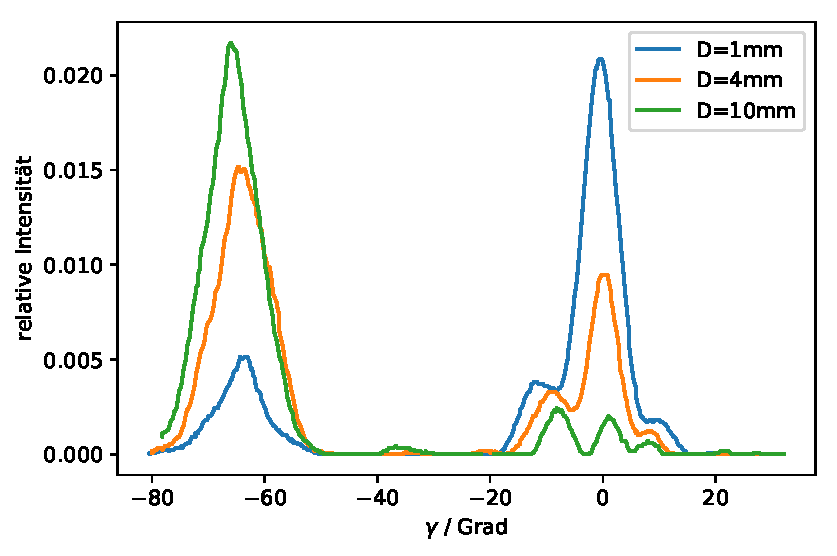
\includegraphics[scale=1]{Bilder/FTIR_Rohdaten.pdf}
	\caption{Intensit"aten der transmittierten Welle bei $\gamma\approx0$ und der reflektierten Welle bei $\gamma\approx\ang{-65}$}
	\label{FTIR_Rohdaten}
\end{figure}
\begin{figure}
	\centering
	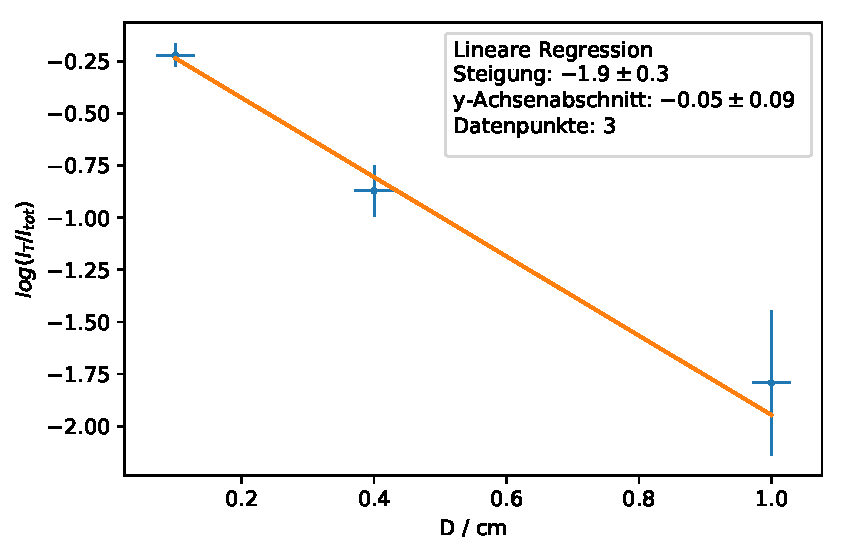
\includegraphics[scale=1]{Bilder/FTIR_LinReg.pdf}
	\caption{Lineare Regression zur FTIR in PE}
	\label{FTIR_LinReg}
\end{figure}
\begin{figure}
	\centering
	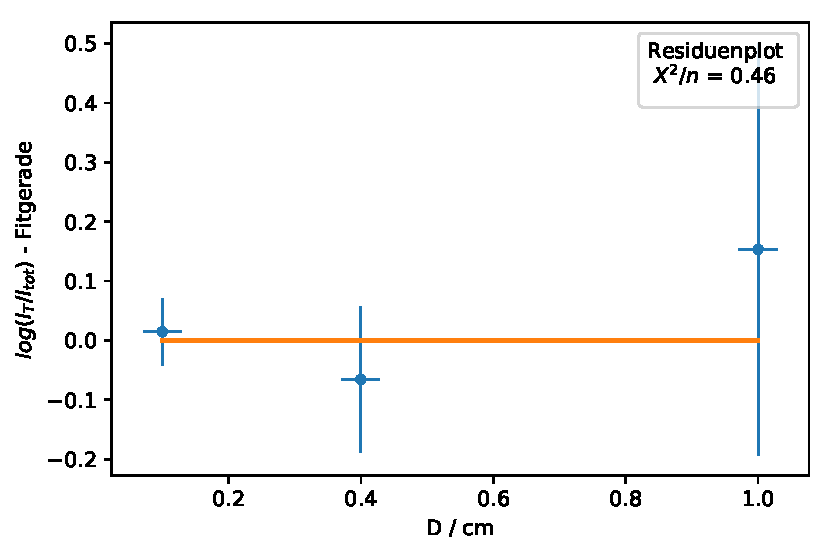
\includegraphics[scale=1]{Bilder/FTIR_Residuen.pdf}
	\caption{Residuenplot zur FTIR in PE}
	\label{FTIR_Residuenplot}
\end{figure}
\end{document}